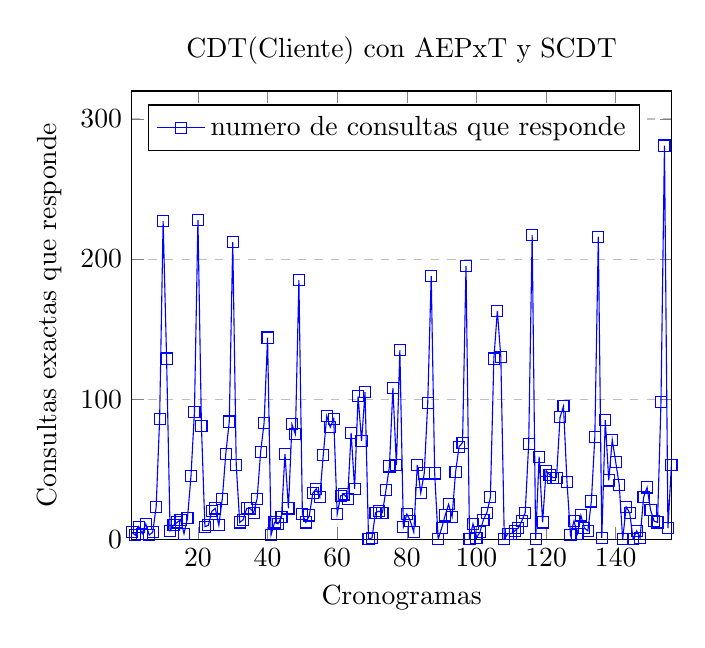
\begin{tikzpicture}
\begin{axis}[
    %CDT = carga de trabajo
    %AEPxT = Algoritmo de Envergadura Probabilista con tiempo de espera
    %SCDT = Seleccion por Carga De Trabajo
    title={CDT(Cliente) con AEPxT y  SCDT},
    xlabel={Cronogramas},
    ylabel={Consultas exactas que responde},
    xmin=1, xmax=156,
    ymin=0, ymax=320,
    xtick={},
    ytick={},
    legend pos=north west,
    ymajorgrids=true,
    grid style=dashed,
]

\addplot[
    color=blue,
    mark=square,
    ]
    coordinates {
   %CARGA DE TRABAJO CLIENTE
   (1,5)
(2,3)
(3,9)
(4,4)
(5,11)
(6,3)
(7,5)
(8,23)
(9,86)
(10,227)
(11,129)
(12,6)
(13,10)
(14,12)
(15,14)
(16,4)
(17,15)
(18,45)
(19,91)
(20,228)
(21,81)
(22,9)
(23,10)
(24,20)
(25,22)
(26,10)
(27,29)
(28,61)
(29,84)
(30,212)
(31,53)
(32,12)
(33,14)
(34,22)
(35,22)
(36,19)
(37,29)
(38,62)
(39,83)
(40,144)
(41,3)
(42,12)
(43,11)
(44,16)
(45,61)
(46,22)
(47,82)
(48,75)
(49,185)
(50,18)
(51,12)
(52,17)
(53,33)
(54,36)
(55,30)
(56,60)
(57,88)
(58,80)
(59,86)
(60,18)
(61,31)
(62,32)
(63,29)
(64,76)
(65,36)
(66,102)
(67,70)
(68,105)
(69,0)
(70,1)
(71,19)
(72,20)
(73,19)
(74,35)
(75,52)
(76,108)
(77,53)
(78,135)
(79,9)
(80,18)
(81,13)
(82,5)
(83,53)
(84,33)
(85,47)
(86,97)
(87,188)
(88,47)
(89,0)
(90,8)
(91,17)
(92,25)
(93,16)
(94,48)
(95,66)
(96,69)
(97,195)
(98,0)
(99,11)
(100,1)
(101,5)
(102,14)
(103,19)
(104,30)
(105,129)
(106,163)
(107,130)
(108,0)
(109,4)
(110,4)
(111,6)
(112,8)
(113,13)
(114,19)
(115,68)
(116,217)
(117,0)
(118,59)
(119,12)
(120,49)
(121,46)
(122,44)
(123,44)
(124,87)
(125,95)
(126,41)
(127,3)
(128,13)
(129,4)
(130,17)
(131,8)
(132,6)
(133,27)
(134,73)
(135,216)
(136,1)
(137,85)
(138,42)
(139,71)
(140,55)
(141,39)
(142,0)
(143,23)
(144,19)
(145,0)
(146,6)
(147,1)
(148,30)
(149,37)
(150,21)
(151,13)
(152,12)
(153,98)
(154,281)
(155,8)
(156,53)
(157,126)
    };
    \legend{numero de consultas que responde}

\end{axis}
\end{tikzpicture}